\newpage

\section{Problem description \& Hypothesis}
As we saw in the state-of-the-art section, we can extract knowledge from mobile communications dataset. This, the solution proposed in this paper is built upon the hypotheses of mobility patterns to predict common and well-known, geographical and time-based patterns to manage roads and infrastructures in a correlated way with the results figured out.
\\
\\
The figure below shows a theoretical commuting model proposed as a main pattern. 
\\
The model shows two peaks, $p_1$ in the range $[7, 8]$ and $p_2$ in $[17, 18]$. This first approach to modelize this dynamic sets up the same height for both peaks $p_1, p_2$. However, numerical results will show that the height of each peak depends on the day of the week. A central valley is defined between $[9, 16]$, with an uniform displacement distribution.
\\
An ad-hoc mathematical model is defined in the next section in order to confirm this hypothesis, consisting on focusing, filtering and processing the main data to contrast the assumption.
\\
\\
The main idea behind the two main peaks, $p_1, p_2$, and the central valley in the model, is that people cover larger distances in their displacements early in the morning i.e.: $p_1$ related with the common business activity. After the first peak $p_1$, people stay in this target destinations, working, eating, etc ..., but in a more static point of view and always performing displacements. The last point in the hypothesis approach shown in Figure~\ref{fig:commuting} is the second peak $p_2$, when people return to their destination or the last business activites took place.
\\
\\
The geographical behaviour of the proposed dynamic, always mixed with the temporal component, will by contrasted using GIS tools in order to visualize the expansions and contractions in the main points shown by the hyphotesis: $p_1, p_2$ and the central valley: an expansion when the maximum displacement is reached on the first peak $p_1$, and a partial contraction when the central valley is reached. Another displacement expansion when peak $p_2$ is reached and its corresponding contraction around $p_2$, when it is declining.


 
 \begin{figure}[h]
\begin{center}
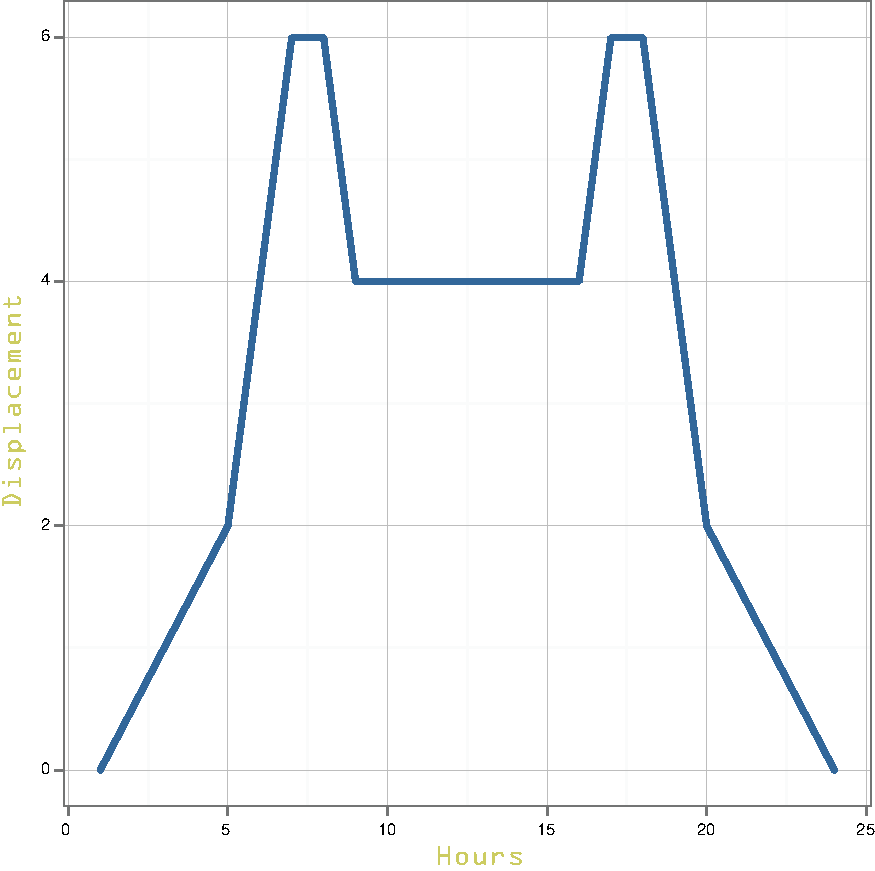
\includegraphics[scale =0.6] {results/images/common_commuting_model.pdf}
\caption{Theoretical Commuting Model}
\label{fig:commuting}
\end{center}
\end{figure}